\documentclass{sigchi}

% Use this command to override the default ACM copyright statement
% (e.g. for preprints).  Consult the conference website for the
% camera-ready copyright statement.

%% EXAMPLE BEGIN -- HOW TO OVERRIDE THE DEFAULT COPYRIGHT STRIP -- (July 22, 2013 - Paul Baumann)
% \toappear{Permission to make digital or hard copies of all or part of this work for personal or classroom use is      granted without fee provided that copies are not made or distributed for profit or commercial advantage and that copies bear this notice and the full citation on the first page. Copyrights for components of this work owned by others than ACM must be honored. Abstracting with credit is permitted. To copy otherwise, or republish, to post on servers or to redistribute to lists, requires prior specific permission and/or a fee. Request permissions from permissions@acm.org. \\
% {\emph{CHI'14}}, April 26--May 1, 2014, Toronto, Canada. \\
% Copyright \copyright~2014 ACM ISBN/14/04...\$15.00. \\
% DOI string from ACM form confirmation}
%% EXAMPLE END -- HOW TO OVERRIDE THE DEFAULT COPYRIGHT STRIP -- (July 22, 2013 - Paul Baumann)

% Arabic page numbers for submission.  Remove this line to eliminate
% page numbers for the camera ready copy
% \pagenumbering{arabic}

% Load basic packages
\usepackage{balance}  % to better equalize the last page
\usepackage{graphics} % for EPS, load graphicx instead
\usepackage[T1]{fontenc}
\usepackage{txfonts}
\usepackage{mathptmx}
\usepackage[pdftex]{hyperref}
\usepackage{color}
\usepackage{booktabs}
\usepackage{textcomp}
% Some optional stuff you might like/need.
\usepackage{microtype} % Improved Tracking and Kerning
% \usepackage[all]{hypcap}  % Fixes bug in hyperref caption linking
\usepackage{ccicons}  % Cite your images correctly!
% \usepackage[utf8]{inputenc} % for a UTF8 editor only


%MC Packages
\usepackage{amsmath}
\usepackage{cite}

% If you want to use todo notes, marginpars etc. during creation of your draft document, you
% have to enable the "chi_draft" option for the document class. To do this, change the very first
% line to: "\documentclass[chi_draft]{sigchi}". You can then place todo notes by using the "\todo{...}"
% command. Make sure to disable the draft option again before submitting your final document.
\usepackage{todonotes}

\newcommand{\jeff}[1]{\textcolor{red}{JMH: #1}}

% Paper metadata (use plain text, for PDF inclusion and later
% re-using, if desired).  Use \emtpyauthor when submitting for review
% so you remain anonymous.
\def\plaintitle{Regression by Eye: Estimating Trends\\in Bivariate Visualizations}
\def\plainauthor{Removed for Review}
\def\emptyauthor{}
\def\plainkeywords{Information Visualization, Graphical Perception, Regression}
\def\plaingeneralterms{Visualization}

% llt: Define a global style for URLs, rather that the default one
\makeatletter
\def\url@leostyle{%
  \@ifundefined{selectfont}{
    \def\UrlFont{\sf}
  }{
    \def\UrlFont{\small\bf\ttfamily}
  }}
\makeatother
\urlstyle{leo}

% To make various LaTeX processors do the right thing with page size.
\def\pprw{8.5in}
\def\pprh{11in}
\special{papersize=\pprw,\pprh}
\setlength{\paperwidth}{\pprw}
\setlength{\paperheight}{\pprh}
\setlength{\pdfpagewidth}{\pprw}
\setlength{\pdfpageheight}{\pprh}

% Make sure hyperref comes last of your loaded packages, to give it a
% fighting chance of not being over-written, since its job is to
% redefine many LaTeX commands.
\definecolor{linkColor}{RGB}{6,125,233}
\hypersetup{%
  pdftitle={\plaintitle},
% Use \plainauthor for final version.
%  pdfauthor={\plainauthor},
  pdfauthor={\emptyauthor},
  pdfkeywords={\plainkeywords},
  bookmarksnumbered,
  pdfstartview={FitH},
  colorlinks,
  citecolor=black,
  filecolor=black,
  linkcolor=black,
  urlcolor=linkColor,
  breaklinks=true,
}

% create a shortcut to typeset table headings
% \newcommand\tabhead[1]{\small\textbf{#1}}

% End of preamble. Here it comes the document.
\begin{document}

\title{\plaintitle}

\numberofauthors{2}
\author{%
%  \alignauthor{Michael Correll\\
%    \affaddr{University of Washington}\\
%    \email{mcorrell@cs.washington.edu}}\\
%  \alignauthor{Jeffrey Heer\\
%    \affaddr{University of Washington}\\
%    \email{jheer@cs.washington.edu}}\\
}

\maketitle

\begin{abstract}
Observing trends and predicting future values are common tasks for viewers of bivariate data visualizations. As many charts do not explicitly include trend lines or related statistical summaries, viewers often visually estimate trends directly from a plot. How reliable are the inferences viewers draw when performing such \emph{regression by eye}? Do particular visualization designs or data features bias trend perception? We present a series of crowdsourced experiments that assess the accuracy of trends estimated using regression by eye across a variety of bivariate visualizations, and examine potential sources of bias in these estimations. We find that viewers accurately estimate trends in many standard visualizations of bivariate data, but that both visual features (e.g., ``within the bar'' bias) and data features (e.g., the presence of outliers) can result in visual estimates that systematically diverge from standard least-squares regression models.
% In most cases regression by eye performs similarly to ordinary least squares regression, but there are edge cases where perceptual and statistical regression systematically diverge. These results suggest that, while regression by eye can be a reliable way of estimating trends, in some common cases these estimates systematically differ from statistical methods of regression.
% JEFF: These last two lines largely re-state the preceding sentence. Maybe add a new line to the abstract that summarizes implications for visualization designers or tool makers.
\end{abstract}

\category{H.5.2}{Information Interfaces and Presentation
  (e.g., HCI)}{Evaluation/Methodology}

\keywords{\plainkeywords}

\newcommand{\outlierFig}{
  \begin{figure}
  \centering
  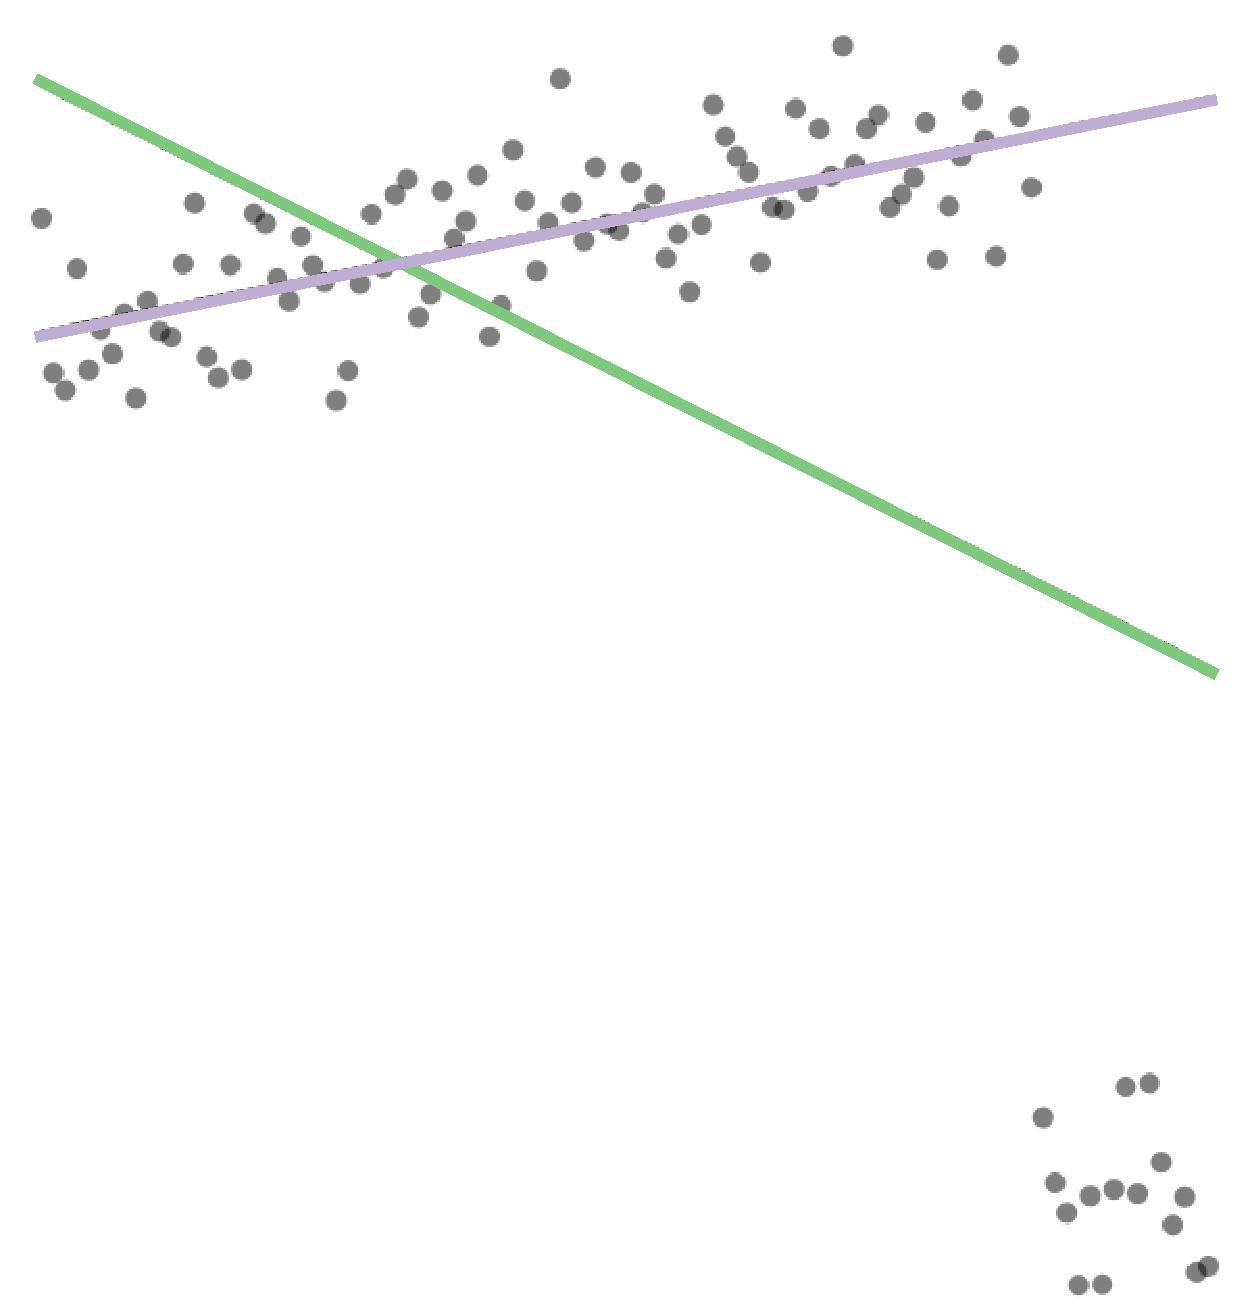
\includegraphics[width=.55\columnwidth]{figures/exp4}
  \caption{A cropped example stimulus from experiment 3. We replaced the final 15 points of this dataset with extreme values. The overlaid purple trend line represents a robust OLS fit (ignoring the outlier values), while the overlaid green line represents the fit with all points included. Participants' estimates of trend lines were universally closer to the robust than the non-robust trend; regression by eye tends to underweight outliers compared to OLS. \jeff{Could we include the average trend line produced by participants?}}
  \label{fig:outlier}
  \end{figure}
}

\newcommand{\expFig}{
  \begin{figure}
  \centering
  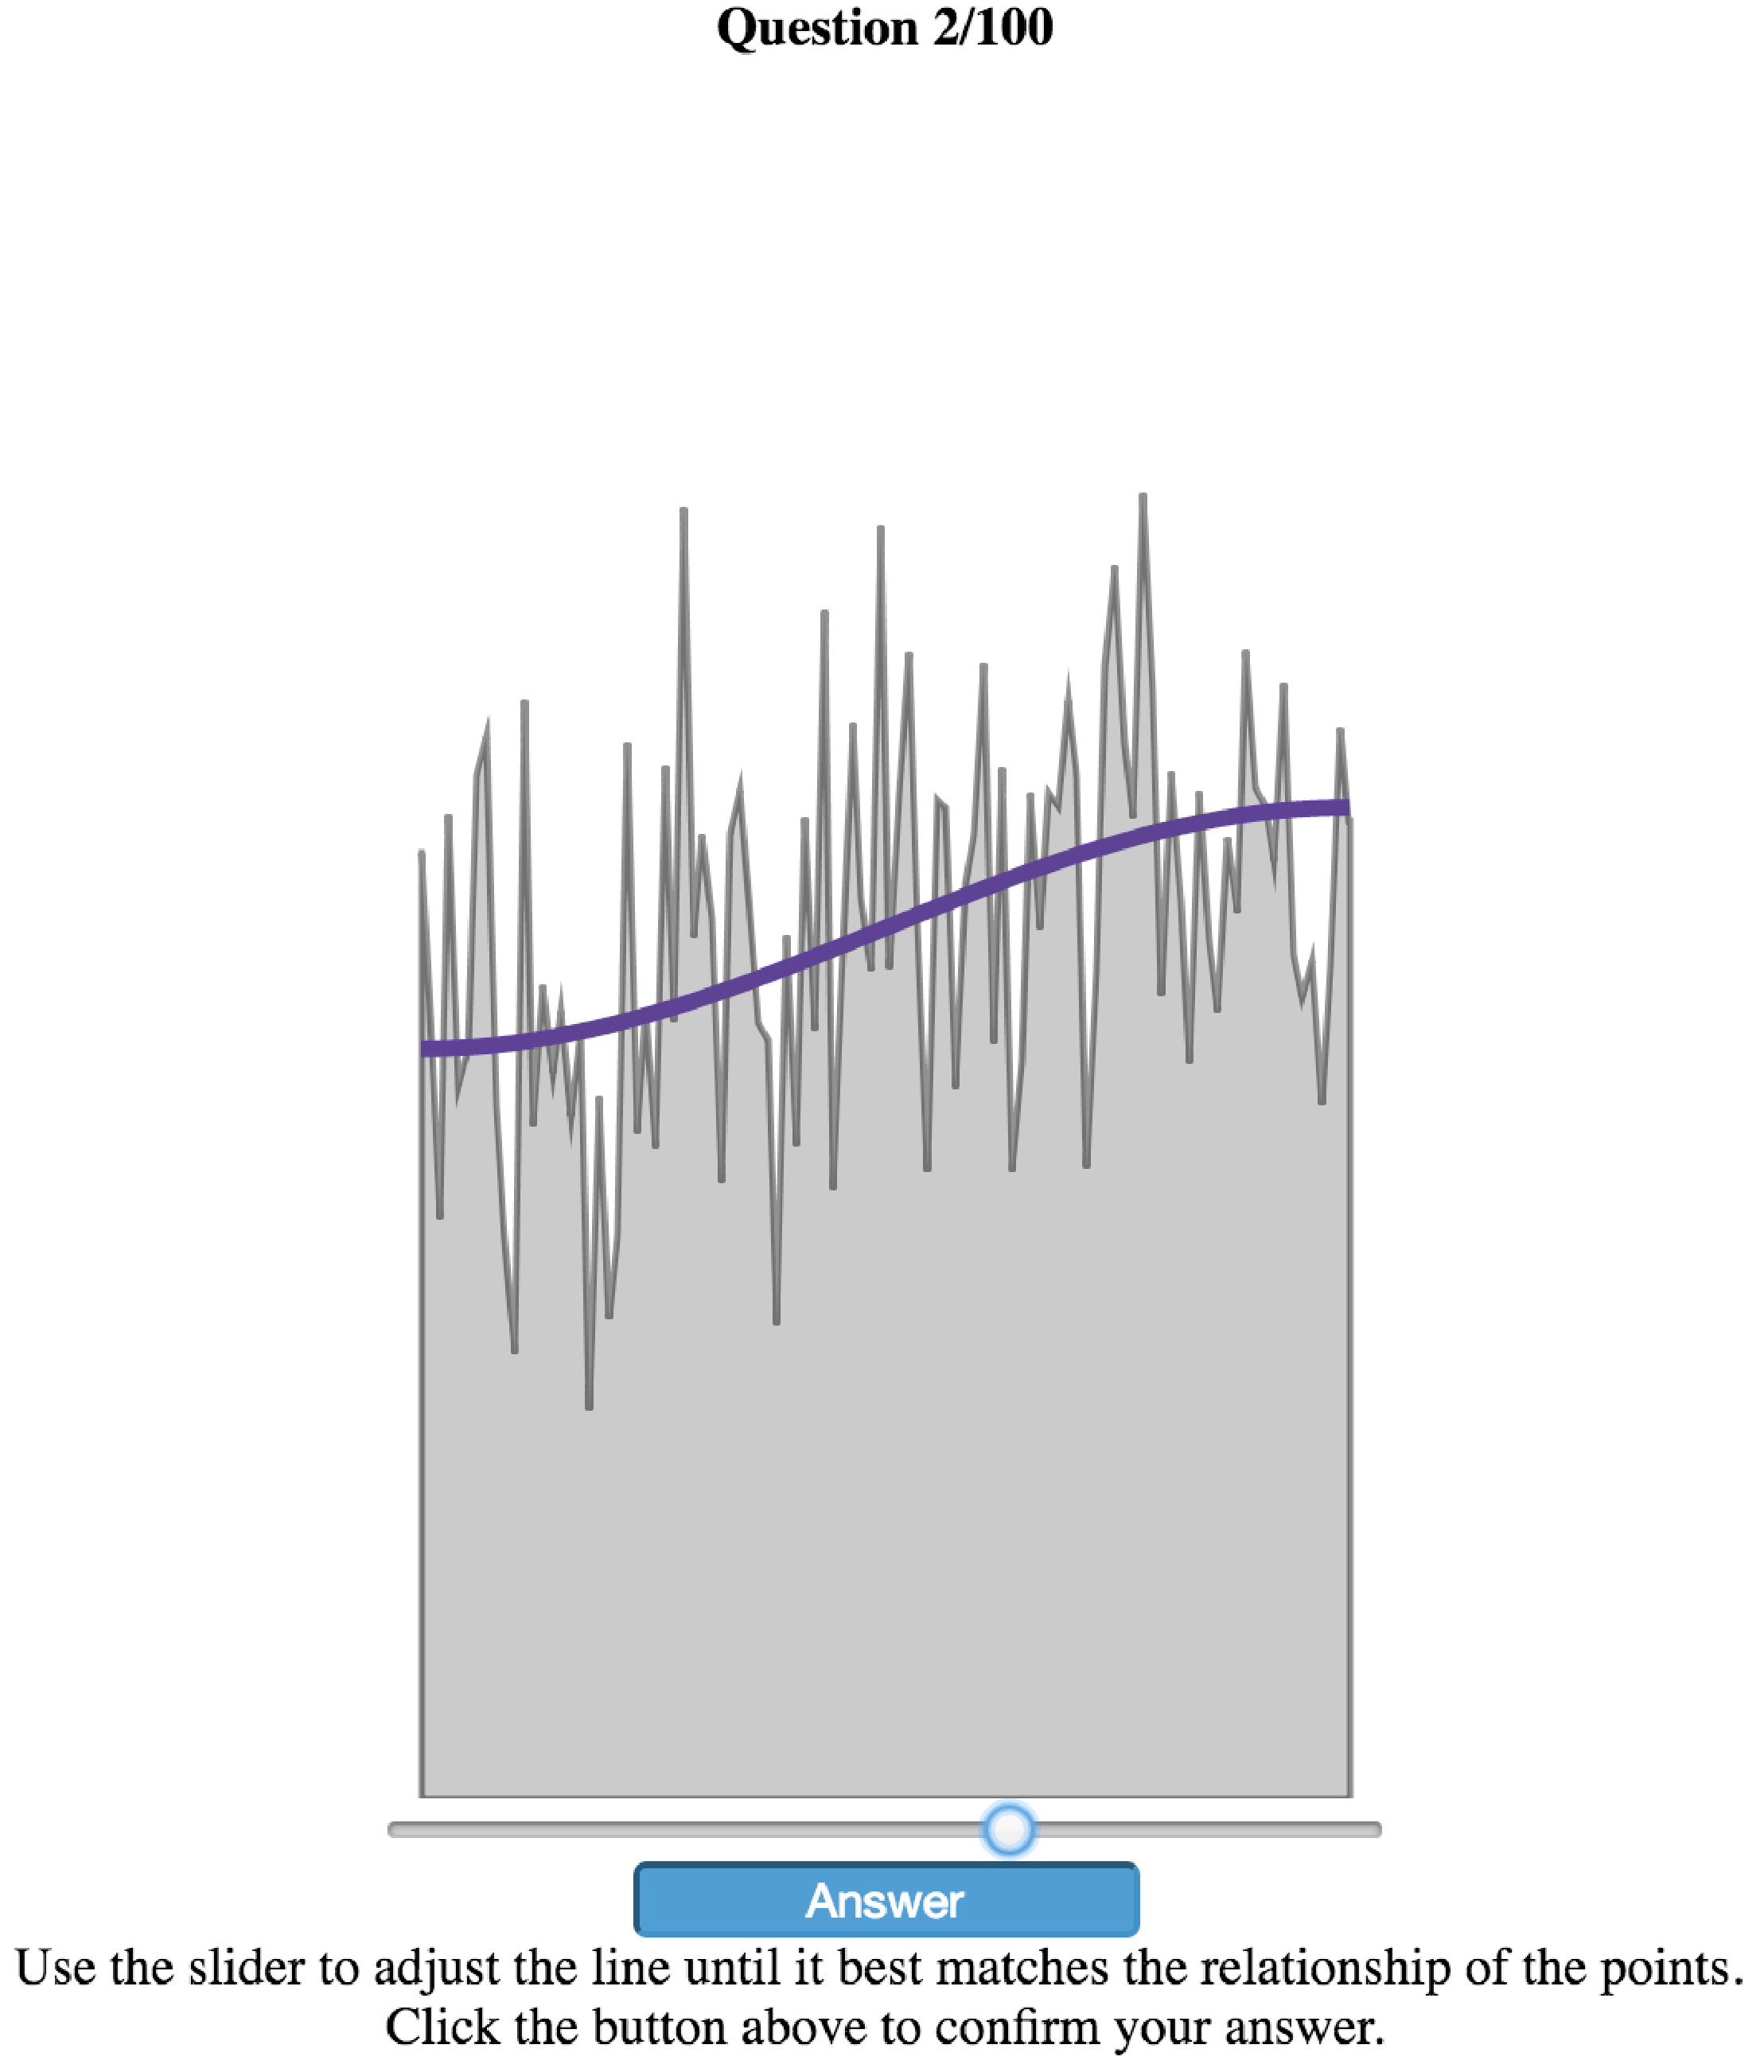
\includegraphics[width=.65\columnwidth]{figures/exp}
  \caption{An example estimation task from our experiments. Here, the participant must adjust the amplitude of the purple trigonometric function until it best matches a particular set of bivariate data.}
  \label{fig:experiment}
  \end{figure}
}

\section{Introduction}
\anscombeFig

An oft-cited example of the power of data visualization is Anscombe's quartet~\cite{anscombe1973graphs}: a set of four bivariate datasets with identical summary statistics, but with qualitatively different patterns when drawn as four scatter plots (Fig. \ref{fig:anscombe}). This example relies on the fact that people have the ability to \emph{perceptually} estimate \emph{statistical} quantities of interest. Visualization users regularly perform statistical tasks\,---\,including model selection, identification of outliers, and estimation of summary statistics\,---\,entirely through visual inspection. Recent work examines the accuracy of visual estimation of means in scatter plots \cite{gleicher2013perception} and time series data \cite{correll2012comparing}, and speculates on the affordances of visualizations in general for supporting visual estimation of summary statistics \cite{szafir2016four}.

The estimation of trends in bivariate data is an important analytical task, as it is the basis for many factors relevant to decision-making, such as prediction, imputation, and comparison. However, model information is not always explicitly included by visualization designers. When designers do include trend information (for instance, by annotating a scatter plot with a line of best fit), other statistics relevant to the model (such as $r$ values or confidence bands) may be absent. Viewers must therefore perform visual estimation to gain a sense of any relevant statistics not provided.

Even if designers include modeling information, the audience may lack the statistical expertise to interpret these values, or may be misled if the data violate modeling assumptions. As a further complication, the form of visual encoding may influence viewers' inferences. For instance, viewers may be more likely to consider trends with line charts, and to compare individual values with bar charts \cite{zacks1999bars}. Visual design choices can also introduce bias, such as the visual asymmetry of bars causing ``within-the-bar'' bias \cite{newman2012bar}. Designers would benefit from guidance regarding how accurately viewers make trend estimations by eye, and to what degree different visualization types might bias these estimations.

Knowing the strengths and limitations of such ``estimation by eye'' is therefore important for designers of data visualizations seeking to communicate statistical quantities, especially to a general audience. On the one hand, visual estimations may be \emph{inaccurate} for the use cases intended by a designer, or they may be \emph{biased}, leading to systematic over- or under-estimations. On the other hand, while visual estimation lacks the precision of formal statistics, it may be relatively unencumbered by modeling assumptions.

In this work, we describe a series of crowdsourced experiments on the visual estimation of trends in common bivariate visualizations such as scatter plots, area charts, and line graphs. We present the results of three studies investigating estimation of trend slope, trend intercept, and the effect of outliers. We find that, while in most cases viewers accurately estimate trends, area charts introduce systematic under-estimation of trend intercept, and that viewers give low weights to extreme values when estimating trends. These results suggest that there are several areas where human judgments diverge from the fitted models generated by techniques such as Ordinary Least Squares (OLS), and that the design of bivariate visualizations can introduce additional biases in these judgments.

Designers should therefore make an informed decision between designing for regression by eye and the explicit annotation of statistical regression information. Regression by eye affords quick estimations and flexibility in model selections, but is subject to perceptual biases and inaccuracies in estimation. Explicit annotation affords accuracy, but constrains the model space, and adds visual complexity to plots.

\section{Related Work}

While there is a great deal of foundational work in visualization and graphical perception dealing with the estimation of individual values in visualizations (such as the height of the bar in a bar chart, or the angle of a line in a line graph), there is comparatively little work on how viewers of visualizations perceive aggregate statistical quantities.

Ariely~\cite{ariely2001seeing} suggests that, in concert with the perception of individual objects, we also collect information about the \emph{ensemble} properties of visual displays. Szafir et al.~\cite{szafir2016four} note that this \emph{ensemble coding} might afford relatively accurate estimation of \emph{summary statistics} in visualizations. However, visualizations with good performance for summary tasks may not result in good performance at point tasks, and vice versa~\cite{albers2014task,fuchs2013evaluation}. A further difficulty is that tasks requiring estimation of values in visualizations (where there is a single correct answer) are qualitatively different from tasks requiring predictions (where differing mental models and priors can result in a multitude of potential valid responses).

Scatter plots are a standard means of visualizing bivariate data, with a multitude of design parameters that affect their suitability for aggregate tasks~\cite{cleveland1984many}. Prior work has confirmed that viewers can make use of scatter plots to perform prediction tasks (which tacitly rely on trend estimation) in ways that are robust to both noise~\cite{harvey1997effects} and problem frame~\cite{lewandowsky2011popular}. However, the heuristics used to perform these prediction tasks (such as the anchor-and-adjust method~\cite{bolger1993context}) can introduce biases.

Similarly, visual design choices (for instance, the decision to encode class membership with color or with shape) can also impact performance at aggregate tasks~\cite{gleicher2013perception,lewandowsky1989discriminating}. The aspect ratio of graphs can also bias judgments about trends~\cite{beattie2002impact}, as wider aspect ratios can cause viewers to underestimate the severity of effects, when compared to narrower charts. Another bias in prediction tasks is the ``within-the-bar'' bias \cite{newman2012bar}: for visually asymmetric visualizations such as bar charts, points contained within the visual area of the bar glyph are perceived as likelier than those outside the glyph.

Recent work in the visualization community has focused on the perception of correlation in scatter plots. Rensink et al.~\cite{rensink2010perception} show that viewers can estimate correlation with some accuracy in scatter plots. Harrison et al.~\cite{harrison2014ranking} extend this finding to other visualization types, and a re-analysis by Kay \& Heer~\cite{kay2016beyond} indicates that, for many of the more esoteric bivariate visualizations, performance at this task is poor. Estimation of correlation can also be biased by the choice of axis scales~\cite{cleveland1982variables}: the whitespace changes introduced by expanding the scale of the axes can cause over-estimation of correlation.

Our task of trend estimation combines elements of both prediction and correlation estimation tasks. As with prediction, there is not necessarily an unambiguous correct estimation of trend (different modeling and regression methods can produce different trend lines). As with correlation, viewers must make holistic judgments about the dataset in a way that (as per Harrison et al.~\cite{harrison2014ranking}) likely relies on a set of visual proxies. That is, while viewers are unlikely to directly estimate correlation \emph{per se}, they are estimating correlation through the perception of visual features such as the envelope of the points, point dispersion, or some other visual feature(s) highly correlated with the statistic of interest.

Prior work in visualization has not directly addressed the capabilities of regression by eye, instead assuming as a given that visual estimates of trend are sufficiently accurate. Work in the perception of summary statistics lends credences to this assumption, but we believe that trend estimation can be biased through conscious or unconscious design choices. For instance, within-the-bar bias may result in under-estimation of trends in bar and area charts, and factors that affect perception of correlation (such as aspect ratio and whitespace) may result in up- or down-weighting of outliers.

\section{General Experimental Methods}

\expFig

In order to assess the ability of visualization viewers to estimate trends, we conducted a series of three crowdsourced experiments on Amazon's Mechanical Turk. We designed these experiments to establish a performance baseline for regression by eye, and to examine potential sources of bias. Crowdsourced graphical perception experiments have been found to produce results that are largely in keeping with prior, lab-based work~\cite{heer2010crowdsourcing, talbot2014four}. In this section, we describe experimental design aspects shared across all experiments.

\subsection{Participants}

We limited the Mechanical Turk participant pool to subjects from within the United States, with a prior task approval rating of at least 90\%. For validation, additional trials, without ambiguities such as outliers or design differences, contained the actual (OLS) trend line, which subjects then needed to simply match.  We excluded the results of participants with average error greater than 0.2 (20 times the step size of the slider) on these validation questions. Across the three reported experiments and pilots, we performed 7 such exclusions. We recruited additional participants to replace these excluded subjects. Based on timings from internal piloting, we paid each participant \$2 for their participation, for a target rate of \$8/hour.

We analyzed data from 48 participants for each experiment (excluding rejections), for a total of 144 participants (98 male, 43 female, 3 who declined to state; $\mu_{age}= 33.2$, $\sigma_{age}=8.8$). Across the subject pool, 10 reported having graduate or professional degrees, 69 college degrees, 40 at least some college, and 25 high school diplomas. After completing the main experimental task, participants were asked to self-assess their familiarity with charts and graphs on a 5 point Likert scale. The plurality (64) rated themselves as ``3. Some familiarity,'' and none rated themselves with the maximum rating of ``5. A great deal of experience.''

\subsection{Experimental Interface}
\typesFig

We investigated three types of common bivariate visualizations: scatter plots, line graphs, and area charts (see Fig. \ref{fig:types}). In each experiment, we presented participants with a visualization and asked them to interactively adjust trend lines to best fit the data.  Participants responded using a slider without tick marks, in order to limit anchoring effects~\cite{matejka2016effect}. Moving the slider adjusted a purple trend line by modifying its slope (in experiments 1 and 3) or its y-intercept (in experiment 2). Fig. \ref{fig:experiment} shows an example experimental task. After moving the slider, participants had to confirm their choice of trend line. The primary dependent measure is accuracy (e.g., the difference between the subject-specified slope and the slope of the series if the residuals were removed). We chose this design over a standard binary forced choice design for its greater expressiveness, as well as for the interactive feedback of adjusting the fit by hand. We avoided more expressive designs (such as freeform drawing) in order to constrain the model space and to reduce the impact of factors such as noise from motor movements or heterogeneous input devices.

\subsection{Data Generation}

\sigmasFig

\trendtypesFig

For each stimulus we wished to have precise, independent control over relevant statistics such as noise, slope, and sample size, while maintaining the appearance of a ``natural'' distribution of points. Existing methods for generating points for related experimental tasks such as estimation of correlations (e.g., Harrison et al.~\cite{harrison2014ranking}) do not afford independence: e.g., Pearson's $r$ is correlated with the slope, as points with identical residuals but different slopes of their linear fits will have differing $r$ values. We also wished to have a fair comparison between visual estimation and the results of ordinary least squares (OLS) regression. We therefore used the standard model of OLS to generate points, namely that $y=\beta x + \epsilon$, where $\epsilon$ is a normally-distributed error term.

For each point set, we placed 100 points along a particular trend, regularly spaced in x. This both affords the use of linegraphs and area charts for displaying this data (as they require that points be one to one), and aligns well with time series data, a common domain for estimating (temporal) trends and relationships. For each point set, we created a set of residual values, sampled evenly from a Gaussian. The bandwidth of this Gaussian controls both goodness of fit and dispersion of points (see Fig. \ref{fig:sigmas}). We permuted this set of residuals, and then applied them to the original points. As heteroskedasticity introduced through permutation could alter the actual trend away from the target trend, we performed rejection sampling to ensure that the trend of the resulting points were within $10^{-7}$ of the target trend. We reused these residuals across all different trend types (linear, quadratic, or trigonometric). Fig. \ref{fig:trendtypes} shows these different trend types on the same set of residuals.

Except where noted, we selected trend lines that were centered in the image: that is, for a horizontal data extent of $[0,1]$, $f(0.5) = 0.5$. In all experiments, we desired control over the direction of the trend. For linear fits, this is the slope of the trend line. For quadratic fits, this was the curvature, as controlled by the coefficient of the second degree term. For trigonometric fits, this was the amplitude of a cosine function (with negative amplitude corresponding to negative slopes). These terms create similar relationships, such that a value of $0$ is the line $f(x)=0.5$, a value of $1$ goes from $f(0)=0$ to $f(1)=1$, and $-1$ has the inverse relationship.


\section{Experiment 1: Slope Estimation}

We designed our first experiment to examine how accurate participants were at estimating the magnitude (slope, amplitude, or curvature) of trends in bivariate visualizations. We examined three types of bivariate visualizations: scatter plots, line graphs, and area charts (with the filled area below the line). In addition to linear trends, we examined more complex relationships such as quadratic and trigonometric functions.

We presented participants with a series of bivariate visualizations, who adjusted a slider to fit the perceived trend. The slider parameterized one of three types of trend: linear, quadratic, or trigonometric. For each stimulus, participants adjusted a slider that controlled the slope of a rendered trend line. In the case of quadratic trends, this slope was the curvature; for trigonometric fits, the positive/negative amplitude.

Participants saw one of each combination of 3 chart types (scatter plot, line graph, or area chart), 8 possible slopes $\beta = \pm \{0.1,0.2,0.4,0.8\}$, and 4 bandwidths of Gaussian residuals $\sigma = \{0.05,0.1,0.15,0.2\}$, for a total of 96 stimuli. We also included an additional 4 validation stimuli otherwise excluded from analysis. The type of trend (linear, quadratic, or trigonometric) was a random factor, with 32 stimuli of each factor level randomly assigned.

\subsection{Hypotheses}

We had three hypotheses for the first experiment:
\begin{enumerate}
	\item \textbf{As the bandwidth of the residuals increased, accuracy would decrease}. Increasing the bandwidth of the residuals results in a lower correlation coefficient and higher perceived noise in the bivariate data. Prior work indicates that these related measures correspond to decreased accuracy for aggregate tasks in bivariate visualizations~\cite{albers2014task, harrison2014ranking}.
	\item \textbf{More complex relationships would result in lower accuracy}. Quadratic and trigonometric relationships are visually more complex than linear relationships, and often require more complex statistical methods to analyze. We anticipated that estimation of these less familiar relationships would therefore be more difficult than the linear case.
	\item \textbf{Estimations would be unbiased}. That is, there would be no systematic over- or under-estimation of trends.
\end{enumerate}

\subsection{Results}

\expOnesigmasFig

\expOnetypesFig

We performed a three-way analysis of covariance (ANCOVA) of the effect of residual bandwidth, graph type and trend type on error in estimation of trend lines. We included participant ids and the actual slope of the trend line as covariates. We defined error as the absolute difference between the slope of the OLS trend line, and the slope of the participant estimate.

In this experiment, the primary measure of performance was the interquartile mean (or midmean) of absolute error. The interquartile mean discards points in the first and fourth quartiles before averaging, trimming the tails of distributions. Cleveland \& McGill~\cite{cleveland1984graphical} used the interquartile mean to provide a more robust measure of central tendency for responses from graphical perception studies, where participant error can create long tailed distributions of error. This is especially the case for crowdsourced studies, where correcting for data quality issues is perceived as more difficult than in laboratory settings~\cite{heer2010crowdsourcing}.

Our results support our first hypothesis: \textbf{larger residuals reduce accuracy at regression by eye}.  We observed a significant main effect for the bandwidth of the Gaussian used to generate residuals ($F(1,4554)=950$, $p<0.001$). The interquartile mean of absolute error increased monotonically with this bandwidth, from $0.02$ of the actual slope of the trend line when the bandwidth was $0.05$, to $0.12$ when the bandwidth was $0.20$. Figure \ref{fig:exp1sigmas} illustrates this result.

Our results fail to support our second hypothesis: \textbf{there was no statistically significant difference in estimation accuracy among linear, quadratic, or trigonometric trends}. Fit type had only a marginal main effect ($F(2,4554)=2.60$, $p=0.074$), and post-hoc tests (using Tukey's Honest Significant Difference) did not identify any significant pairwise interactions. The interquartile mean of absolute error of was $0.06$ for linear and quadratic fits, and $0.07$ for trigonometric fits (see Fig. \ref{fig:exp1types}). This result suggests that the relative unfamiliarity of non-linear trends does not have a notable impact on performance.

Our results support our third hypothesis: \textbf{there was no statistically significant bias in estimations}. Participants saw a balanced set of positive and negative trends. If estimates of these trends were unbiased, we would expect the average signed error to be close to zero. The average signed error was $0.0008$, far less than the fidelity of the slider used to input guesses ($\Delta=0.01$). A Student's T-test failed to support the hypothesis that $mu_{error}\ne0$ ($t(4590) = 0.39$, $p=0.70$).

%The average absolute error of slope estimation across all conditions had an interquartile mean of $0.06$ for slope values ranging from $\{-1,1\}$, corresponding to an error rate of $17\%$ of the actual slopes. 
As a point of comparison, the interquartile mean of the absolute log error, calculated as per Cleveland \& McGill~\cite{cleveland1984graphical} ($log_2 |\text{error}| + \frac{1}{8}$) was $2.4$ across all conditions. This is comparable to the error rates of many other graphical perception tasks as observed in both lab and crowdsourced studies. For instance, Heer \& Bostock~\cite{heer2010crowdsourcing}  report an absolute log error of $2.5$ for proportional judgments in treemaps, and Cleveland \& McGill~\cite{cleveland1984graphical} report an absolute log error of $2.4$ for proportional judgments in stacked bars (although compare to a log error of estimation of relative lengths of lines of $1.1$). This similarity suggests that, despite requiring estimation of aggregate statistical information, regression by eye results in judgments that are accurate enough for many practical purposes, comparable with the expected accuracy in comparing individual values in visualizations. 

\section{Experiment 2: ``Within-the-Bar'' Bias}

\expTwoTypesFig

``Within the bar'' bias is a known perceptual bias involving bar charts, in which points contained in the visual area of the glyph of the bar are deemed likelier than points outside of the glyph. Newman \& Scholl~\cite{newman2012bar} encountered this bias for a sampling task: ``how likely is this point to have been drawn from the distribution represented by this bar?'' Correll \& Gleicher~\cite{correll2014error} likewise encountered this bias for inferential tasks: ``how likely is the population mean to take a particular value, given the sample represented by this bar?''

We hypothesized that this bias would likewise occur for regression tasks when using visually asymmetric visualizations such as area charts. The slope estimation task in the previous experiment would not capture this bias, as there is no method for participants to indicate a \emph{uniform} under-estimation in trends; decreasing the slope would cause under-estimation at the beginning of the plot but not the end, and vice versa. We therefore designed this experiment to elicit estimates of the y-intercepts of trends. A within-the-bar bias would then appear as systematic under-estimation of intercept in area charts.

As with the previous experiment, we presented participants with a series of bivariate visualizations. However, instead of estimating the \emph{slope} of the points, participants estimated the \emph{y-intercept} of the trend line. For each trial, we added a uniform offset to the points in the bivariate visualization in the data range $[-0.25,0.25]$. The rendered trend line was initially placed with the correct slope, and such that $f(0.5)=0.5$ in data space. Participants adjusted a slider controlling the vertical offset of this trend line.

The plots had the same factor levels as the previous experiment, for a total of 96 stimuli per participant, with an additional 4 validation stimuli otherwise excluded from analysis. The uniform offset was an additional random factor for each stimulus.

\subsection{Hypotheses}

We had one hypothesis for the second experiment:
\begin{enumerate}
	\item \textbf{Area charts would be subject to within the bar bias.} That is, participants would estimate lower values of y-intercepts of trends than with line graphs and scatter plots.
\end{enumerate}

\subsection{Results}
We performed a one-way ANCOVA of the effect of graph type on \emph{signed} error. We included residual bandwidth as a covariate, and participant ids as a random factor.

Our results support our first hypothesis: \textbf{participants systematically underestimated the intercept of trends in area charts, but not in scatter plots or line graphs}. We observed a significant main effect of graph type on signed error ($F(2,2431)=27$, $p<0.001$). A post-hoc Tukey's HSD confirmed significant differences in error between the area chart and the other two chart types, but not between scatter plots and line graphs. The interquartile mean of the signed error of estimations made with area charts was an under-estimation of $-0.02$, compared to an interquartile mean of $0.002$ for the other two conditions. This under-estimation corresponds to unsigned errors more than twice as large in area charts (interquartile mean of $0.04$ for intercepts that ranged from $\{-0.25,0.25\}$, compared to $0.02$ for line graphs and scatter plots). Figure \ref{fig:exp2types} illustrates this result.

\section{Experiment 3: Estimation Involving Outliers}

\outlierFig

\outliersFig


OLS regression operates under the assumption that there is a unimodal, symmetric distribution of residuals surrounding the line of best fit. Extreme outliers violate this assumption, and can result in trend lines that are substantially different from those produced by more robust methods. Visual inspection can accurately identify certain classes of outliers~\cite{albers2014task}. Therefore, regression by eye may afford the estimation of both outlier-robust and outlier-sensitive trends. However, cognitive biases~\cite{tversky1975judgment} such as anchoring (the tendency to overweight the first set of information), availability (the tendency to overweight more recent or extreme information), and the hot-hand fallacy (the tendency to assume that trends of high or low values will continue) can impact how viewers categorize and utilize outliers in prediction tasks~\cite{campbell2009anchoring, ji2001culture}. In other words, regression by eye may not uniformly weight outliers, depending on their position in the plot.

This experiment was largely identical to Experiment 1, except we designated 0, 5, 10, or 15 points at the very beginning, first third, or end of the series as outliers. We vertically positioned outliers within the top or bottom 10\% of the visual area of the visualization (whichever was farthest from the trend line), and added random jitter. We then calculated the outlier-sensitive line of best fit, as well as the intersection between this new trend line and the original, outlier-less trend line. We refer to the original trend line, estimated without the presence of outliers, as the \textbf{robust trend line}. We refer to the re-estimated trend, which takes into account the added outliers, as the \textbf{OLS trend line}. Figure \ref{fig:outliers} shows examples of this process, and the corresponding changes in trend line.

As in Experiment 1, the participants controlled the slope of a rendered trend line with a slider. However, rather than being placed such that $f(0.5)=0.5$, we offset the trend line to the intersection of the robust (without outliers) and non-robust (including outliers) trend line. This allowed participants to express both types of fit with the same slider interaction, while affording estimations beyond a simple interpolation of both trends. We limited the stimuli to linear fits only, excluding quadratic and trigonometric trends from this experiment.

Participants saw one of each combination of factors: the three graph types, eight slopes, and four Gaussian residual bandwidths. The four outlier quantities $\{0,5,10,15\}$ were an additional factor. To maintain a manageable number of stimuli (piloting showed evidence of fatigue for more than 100 stimuli per trial), both the sign of the trend line (positive or negative), and the location of the outliers (beginning, first third, or end) were random factors, with each level randomly apportioned to half and one third of the stimuli respectively. This resulted in 96 total stimuli, with an additional 4 validation stimuli otherwise excluded from analysis, in line with prior experiments.

\subsection{Hypotheses}

We had three hypotheses for the third experiment:
\begin{enumerate}
	\item \textbf{Participant estimation would hew closer to a robust trend line ignoring outliers, rather than the OLS trend line.} We assumed that in general, participants would ignore or downweight outliers when performing regression by eye.
	\item \textbf{As the number of outliers increased, estimations would be closer to the non-robust OLS fit.} We speculated on the existence of a ``tipping point'' of outlier density, beyond which participants would avoid robust fits, and interpolate between the robust and OLS fits.
	\item \textbf{Outliers at the end of the chart would result in estimations closer to the OLS fit than outliers in other locations on the plot.} Prior work on cognitive biases in predictions suggests that viewers may give more credence to more recent outliers (as indicative as new anchor points, or of an emerging ``streak'')~\cite{croson2005gambler}. We therefore believed that these points would be more heavily weighted, and the resulting estimation closer to the outlier-sensitive OLS line, than outliers ``earlier'' in the plot.
\end{enumerate}

\subsection{Results}

\expThreeErrorFig

\expThreeOutliersFig

Our results support our first hypothesis. \textbf{Participant estimates were closer to the robust trend line than the trend line that included outliers}. Excluding conditions with zero outliers (and so the two trend lines would be identical), the interquartile mean of absolute error was over $4$ times higher when calculated as a comparison to the OLS trend line ($0.36$) as opposed to the robust trend line ($0.08$). A Student's T-test confirmed that the error as defined by the OLS line was significantly higher than the robust line ($t(6670)= 43$, $p<0.001$). However, a Student's T-test found a significant difference in unsigned error when compared to the robust trend line between estimates where no outliers were present, and those with any amount of outliers ($\mu=0.07$ vs. $\mu=0.08$, $t(3808) = 9.8$, $p<0.001$). Figure \ref{fig:exp3errorType} illustrates this result. This indicates that participants are not entirely ignoring outliers, although the small effect size suggests that participants are giving outliers significantly less weight than OLS regression. Figure \ref{fig:outlier} shows an example of this weighting.


Our results fail to support our second hypothesis. \textbf{While participant estimates diverge from the robust line as the number of outliers increases, the OLS trend line diverges faster than participant estimates}. There was a significant positive interaction between outlier count and absolute error with respect to the robust trend line ($R^2 = 0.02$, $F(1,4591)=110$, $p<0.001$). However, there was also a significant positive interaction between outlier count and absolute error with respect to the OLS line  ($R^2 = 0.38$, $F(1,4591)=2800$, $p<0.001$). Additionally, while the range of errors with respect to the robust line remained small (interquartile means of $0.07$ with 0 outliers, monotonically increasing to $0.10$ with 15 outliers), absolute error with respect to the OLS line increased almost 7-fold, from $0.07$ with 0 outliers, monotonically to $0.54$ with 15 outliers. These results indicate that while increased numbers of extreme values may result in participants increasing the weight of these outliers, this increase in weight is slower than the sensitivity of OLS to outliers.  Figure \ref{fig:exp3outliers} illustrates this result.

Our results also fail to support our third hypothesis, and seem to support its inverse: \textbf{There was no significant impact of outlier location on performance}. There is a confound between outlier location and OLS line: outliers on the ends of the data ranges create larger shifts in slope than outliers in the center, which may only create shifts in intercept. To evaluate our third hypothesis, we therefore defined a parameterized performance function $\frac{\text{Estimated Slope}-\text{Robust Slope}}{\text{OLS Slope} - \text{Robust Slope}}$ that contextualizes a participant estimate as an interpolation between the robust slope (value of $0$) and the OLS slope (value of $1$). A one way ANCOVA of this interpolation value as an effect of outlier location, with outlier count as a covariate, and participant ID as a random factor, found no significant effect ($F(2,3441)=0.63$, $p=0.53$).

%Contrary to our hypothesis, outliers in the middle location resulted in guesses that were closer to the trend line (interquartile mean of interpolation value of $0.66$, compared to $0.24$ for outliers at the beginning location, and $0.32$ for outliers in the final location).

\section{Discussion}

In many cases, designers do not explicitly encode regression information. In other cases, viewers may not have the statistical or graphical expertise to interpret such information, even when it is supplied. Yet, our results point to regression by eye as a robust and reasonably accurate method for estimating trends in bivariate data. Participants from a variety of backgrounds and levels of self-reported graphical and statistical expertise were capable of estimating both the slope and intercept of both linear and non-linear trends. That is, viewers of visualization are largely trustworthy when estimating the relationship between two variables in a plot.

However, this general accuracy of trend estimation is not universal. Area charts are visually asymmetrical: the area below the line is filled in, and the area above it is not. We found that this asymmetry creates a within the bar bias: a systematic under-estimation of the intercept of trends, due to the perceived higher likelihood of points in the filled-in area. Designers hoping to rely on regression by eye should avoid such asymmetries in their bivariate visualizations.

Likewise, viewers do not give the same weight to outliers as OLS regression, but they do not ignore them either. For noisy data, this robustness may be beneficial: people can be relied on to perform filtering operations without explicit guidance. In other cases, this insensitivity may be undesirable. For instance, more complicated automatic analytical processes may use OLS regression or other outlier sensitive techniques as part of their calculations, resulting in a disconnect between human and statistical conclusions at later stages of the sensemaking process. Similarly, the human tendency to discount or downweight outliers may result in slow adaptation to new data that does not fit into existing patterns.

\subsection{Limitations \& Future Work}

Our experimental setup was intentionally simple, affording only a single free parameter for each experiment. In actual regression by eye, the viewer may simultaneously engage in multiple types of estimation: choosing a particular type of fit, ignoring outliers, and estimating the parameters of the chosen model. Errors in any one of these steps could compound, resulting in performance worse than our measures, where many of these decisions are fixed. It is also likely that there are many visual features, such as the convex hull of points, or the numerosity of point clouds, that are acting as visual proxies for estimation of the trend. Given the unimodal error function and uniform density of our experimental stimuli, these proxies are useful for estimating the trend line. However, in datasets where internal densities of points may be skewed, or the envelope of point clouds non-informative for estimating central tendency, these visual proxies may introduce biases and confounds in visual estimations.

There are also a number of design decisions not considered in this study that could impact regression by eye. For example, Wood et al.~\cite{wood2012sketchy} have shown that ``sketchiness'' in visualizations can result in skepticism of the data and design. It is possible that outliers could receive less visual (and so statistical) weight as a response to this sort of skepticism. Our stimuli likewise contained a sufficient number of points that bar charts were not a feasible choice of visualization. Given the propensity of bar charts to encourage comparison of individual, rather than aggregate quantities~\cite{zacks1999bars}, it is possible that bar charts of smaller scale bivariate data could promote fitting of local rather than global trends.

Finally, we focused on a simple form of regression, ordinary least squares (OLS), as our standard for measuring accuracy. While our data were constructed to satisfy the assumptions of OLS (with the intentional exception of our outlier experiment), in most real world scenarios OLS is just one tool of many, and analysts must exercise judgment when determining how to fit their data. More complex models may not have ready visual analogues, and data concerning regression by eye may not extend to cover these cases.

Our future work is focused in three areas. First, we wish to examine the impact of annotations relevant to regression (such as confidence bands, error bars, and curve boxplots~\cite{mirzargar2014curve}) on regression by eye. Can sufficient information promote caution in judgments of trend? Second, we wish to examine the impact of different rhetorical framings and presentations on regression by eye. Language from semiotics and rhetoric can provide testable structures for how visualizations are consumed~\cite{hullman2011visualization}: these framings could similarly impact statistical judgments. For instance, outliers from a source that is perceived as credible could be weighted higher than outliers with more suspect provenance. Likewise, preconceptions about the volatility of data from certain domains may color how experts estimate trends. Lastly, we wish to examine techniques for overcoming bias in regression by eye and similar visual estimations of statistical quantities. Cognitive and perceptual biases are difficult to overcome, and may require exploration of novel forms of visualization~\cite{micallef2012assessing}.

\subsection{Conclusion}

In this paper, we examine the ability of visualization viewers to perform \emph{regression by eye}: the visual estimation of trends in bivariate visualizations. We show that viewers without statistical training can reliably estimate both linear and non-linear trends in charts such as scatter plots and line graphs. However, area graphs are subject to a ``within the bar'' bias, leading to estimated trends with lower intercepts than other bivariate visualizations. Regression by eye is also less sensitive to outliers than standard least-squares regression. This decreased sensitivity results in a divergence between trends estimated by viewers, which do not give much weight to extreme outliers, and those trends calculated by regression methods that can be heavily influenced by a few extreme values.


\section{Acknowledgments}

Omitted for review.

% Balancing columns in a ref list is a bit of a pain because you
% either use a hack like flushend or balance, or manually insert
% a column break.  http://www.tex.ac.uk/cgi-bin/texfaq2html?label=balance
% multicols doesn't work because we're already in two-column mode,
% and flushend isn't awesome, so I choose balance.  See this
% for more info: http://cs.brown.edu/system/software/latex/doc/balance.pdf
%
% Note that in a perfect world balance wants to be in the first
% column of the last page.
%
% If balance doesn't work for you, you can remove that and
% hard-code a column break into the bbl file right before you
% submit:
%
% http://stackoverflow.com/questions/2149854/how-to-manually-equalize-columns-
% in-an-ieee-paper-if-using-bibtex
%
% Or, just remove \balance and give up on balancing the last page.
%
\balance{}


% REFERENCES FORMAT
% References must be the same font size as other body text.
\bibliographystyle{SIGCHI-Reference-Format}
\bibliography{sample}

\end{document}

%%% Local Variables:
%%% mode: latex
%%% TeX-master: t
%%% End:
